\section{Model checking Group Announcement Logic}\label{sec:algorithms}
%Describe process of translating logical definitions into pseudocode here, then describe model checker in next chapter

In this section we will describe the process of translating the definitions from the previous chapter into algorithms that will be used in our model checker. 

%\todo{Finskrive alt det her, muligens stykke opp og fordele ut etterhvert som det blir relevant}\\
%Before continuing into the translation of defintions into pseudocode, we want to highlight some key differences between the logical definitions of our models and the data structures used in our application. While models themselves are relatively similar, having a set of states and a set of agents, the equivalence relations for each agent and the valuation function for assessing which propositions are true in which states are somewhat different. Our model-structure in the application instead uses a set of edges, pairs of indistinguishable states and which agents consider them so. Secondly it also flips the valuation function in the sense that while the logical definitions define a function which goes from a proposition to the set of states said proposition holds in, our model checker instead goes from a state and returns the set of propositions that hold in that given state.\\

Going back to our revised semantics behind the group announcement operators in Definition \ref{def:GALsemV2} we can see that once we can determine how to enumerate the set of announceable extensions $\anns{G}$, implementing the semantics behind the group announcement operator is fairly straightforward. However, as our definition of $\anns{G}$ uses the concept of bisimulation contracted models, we will first need to cover how we can check whether states are bisimilar and then apply that check to models as a whole in order to reduce them to their smallest bisimilar structures. 

%the definitions of bisimilar states and bisimulation contraction from  and Definition ??? \todo{Actually write definition of bisimulation contraction and refer to it here}. Starting with bisimilarity in general, we will be using the following algorithm for our implementation of bisimilarity checks.
% Discuss basic components of models, states, edges later?
% Skip over algorithms for basic operators

% Repeat why we need bisimilarity check

\subsection{Enumeration of announcements in single agent cases}

Recall the definition of the semantics behind $\M,s \models \dia{G}\varphi$ in Definition \ref{def:dual}, an informal way of explaining it would be that there exists at least one set of formulas the coalition can announce such that $\varphi$ is true after their announcements. 

Using our definitions of labeling formulas and formula extensions in Definition \ref{def:ext} and \ref{def:label} to look at what kinds of formulas any given agent can announce, we note that the goal is to convey information to the other agents in the system. Therefore we do not need to look at the formulas themselves, but only at what consequence announcing them would have and whether or not the agent is able to announce them. For this reason we will be using the concept of formula extensions from Definition \ref{def:ext} instead of concrete formulas as announcing any given formula will eliminate all states not in that formula's extension from the updated model as defined by the semantics of model updates.

\begin{figure}[h]
	\centering
	\scalebox{1.8}{
		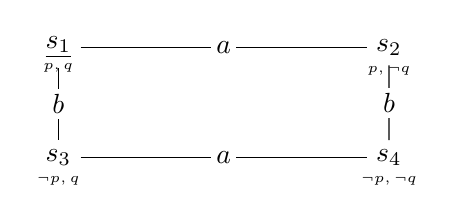
\begin{tikzpicture}[scale = 1.4, every label/.append style = {font=\tiny}]	
				\node[label={[label distance=-0.7cm]:$p,q$}] (s1) at (0,1) {$\underline{s_1}$};
				\node[label={[label distance=-0.7cm]:$p, \neg q$}] (s2) at (3,1) {$s_2$};
				\node[label={[label distance=-0.7cm]:$\neg p, q$}] (s3) at (0,0) {$s_3$};
				\node[label={[label distance=-0.7cm]:$\neg p, \neg q$}] (s4) at (3,0) {$s_4$};
	
				\path[every node/.append style={font=\fontsize{10}{0}, fill=white, inner sep=2pt}] 
					(s1) edge node {$a$} (s2) ++
					(s3) edge node {$a$} (s4) ++
					(s1) edge node {$b$} (s3) ++
					(s2) edge node {$b$} (s4);								
		\end{tikzpicture}
	} %End scaling
	\caption{A basic bisimulation contracted model.}
	\label{fig:GAexample}
\end{figure}

If we attempt to determine which sets of formulas some agent $i$ can announce in the model in Figure \ref{fig:GAexample} we can see that the set of announceable formula extensions will always be a subset of the power set of states in the model. Or more precisely, the set of announceable formula extensions for some agent $i$ in a given pointed model $\M,s$ is a subset of the power set of states in $\M$, where each set is announceable by $i$ if and only if that set follows the following rules in Definition \ref{def:extRules}.

%subset of the power set of extensions of the set of labeling formulas for the model

\begin{definition}[Rules for eliminating formulas by their extension]\hfill
\label{def:extRules}
	For any formula $\varphi$ and bisimulation contracted pointed model $(\M,s)$, the formula's extension in $\M$, $\ext{\varphi}_{\M}$, must satisfy the following rules in order for the formula to be announceable by some agent $i$ in coalition $G$:
	\begin{itemize}
		\item $\ext{\varphi}_\M$ must contain the actual state in our pointed model
		\item $\eqc{s}_a \subseteq \ext{\varphi}_{\M}$
	\end{itemize}
\end{definition}

The reasoning behind these two rules is based on the semantics of the group announcement operators in Definition \ref{def:GALsem}, we can see that we are essentially searching for a combination of formulas which when announced, make $\varphi$ false. Because of this, having an agent announce that they know something which is false, or something they do not actually know, will simply make the public announcement trivially true. This means there is no point in checking any announcement containing such a formula, therefore the formula:

\begin{itemize}
	\item[(1)] has to be satisfied in the `actual' state of our pointed model
	\item[(2)] has to be satisfied in every state the agent is incapable of distinguishing from that `actual' state, meaning the agent's equivalence class for that state must be a subset of the formula's extension in our model
\end{itemize}

\begin{proposition}
For every extension $\ext{\varphi}_{\M}$ that satisfies the rules in Definition \ref{def:extRules} for some agent, any formula with the same extension can be announced by that agent.
\end{proposition}

\begin{proof}
Assuming we have two formulas $\varphi$ and $\psi$, which share the same formula extension, $Ext$, in some pointed model $(\M, s)$, then $\varphi$ is announceable by some agent $a$, iff $\psi$ is, since the formulas hold in exactly the same states, as per the definition of formula extensions.
\end{proof}

From our definition of formula extensions in Definition \ref{def:ext}, the extension of a formula is simply the set of states in which this formula is satisfied. Therefore if $\varphi$ and $\psi$ share the same extension in some model $\M$, then $\M\models\varphi \leftrightarrow \psi$. From this we can further infer that $\M\models K_a\varphi \leftrightarrow K_a\psi$ for every $\psi$ with the same extension as $\varphi$.


\begin{definition}[The set of announceable extensions]\hfill\\
	\label{def:annexts}
	The set of announceable formula extensions $\anns{}$ for some agent $i$, given a bisimulation contracted pointed model $\M,s$ is defined as the following: \\
	$\anns{i,(\M,s)} \subseteq \{\ext{\varphi}_{\M} ~|~ \varphi\in\labels{\M}\}$ where $\ext{\varphi}_\M \in 		     
	\anns{i,(\M,s)}$ iff it follows the rules in Definition \ref{def:extRules}.
	Note that as $\M$ is bisimulation contracted, every formula in $\labels{\M}$ is only satisfied in a single state in $\states$ and every state in $\states$ satisfies exactly one formula in $\labels{M}$. As such, $\{||\varphi||_\M ~|~ \varphi \in \labels{\M}\}$ can be simplified to $\wp(\states)$.
\end{definition}

For a more practical explanation we will apply these rules to the model in Figure \ref{fig:GAexample} for agent $a$. Using $s_1$, denoted $1$ in the next example, as the actual state of our pointed model, we start by generating the power set of states in our model and get the following:

\begin{align*}
	\wp(\states) = \{\emptyset,\{1\},\{2\},\{3\},\{4\},\{1,2\},...,\{1,2,3\},...\{1,2,3,4\}\}
\end{align*}
After applying rule (1) from Definition \ref{def:extRules}	to filter out all formula extensions not containing the actual state of our pointed model we get:
\begin{align*}
	\{\{1\},\{1,2\},\{1,3\},\{1,4\},\{1,2,3\},\{1,2,4\},\{1,3,4\},\{1,2,3,4\}\}
\end{align*}
Applying rule (2) to remove all extensions relating to formulas that $a$ does not know leaves us with:
\begin{align*}
	\{\{1,2\},\{1,2,3,4\}\}
\end{align*}

In other words, given the model in Figure \ref{fig:GAexample} agent $a$ is able to announce any given formula $\varphi$ iff $\ext{\varphi}_{\M,1} \in \{\{1,2\},\{1,2,3,4\}\}$. Therefore, $\anns{a,(\M,1)} = \{\{1,2\},\{1,2,3,4\}\}$.

An interesting thing to note here is that we can combine our labeling formulas with disjunctions to create a formula which is satisfied in any subset of the original set of states we want. So for example, in order to create a formula with the extension of $\{s_1,s_2\}$ all we have to do is put disjunctions between the labeling formulas for $s_1$ and $s_2$ such that $\varphi_{\{s_1,s_2\}} = \varphi_{s_1} \vee \varphi_{s_2}$.

If we then want to apply this to checking whether $\M,s_1 \models \dia{a}K_bp$ where $\M$ is still the model in Figure \ref{fig:GAexample}, then we can see that since $\{s_1,s_2\}\in\anns{a,(\M,s_1)}$ there exists a formula extension that $a$ can announce which would eliminate $s_3$ from the model. Verifying this, we can see that as $\M,s \models K_a\varphi$, announcing this would cause $K_bp$ to be satisfied in the updated model and therefore $\M,s \models \dia{a}K_bp$.

\subsection{Generalizing the single agent case}

Expanding what we have presented so far to encompass coalitions comprised of multiple agents is actually very easy. 
When we are assessing the ability of an agent to announce something which may change the valuation of a formula, we are simply checking whether or not that agent is capable of eliminating certain states in the updated model. In other words, if we wish to assess the ability of a whole coalition, all we need to do is look at which sets of states each agent in the coalition is able to eliminate in unison.

An interesting observation to make is that an agent $i$ is always capable of eliminating any state they can distinguish from the actual state of some pointed model. This means that in order to find out which states a coalition can eliminate, we can simply take the power set of states and limit it to the combinations of states which fit the rules of Definition \ref{def:extRules}, where we slightly tweak rule 2 to the following:

\begin{definition}[The set of extensions announceable by coalitions]
	\label{def:extscoal}
	The set of announceable extensions $\anns{G,(\M,s)}$ for some coalition $G$, given a bisimulation contracted pointed model $\M,s$ is defined as the following: \\
	$\anns{G,(\M,s)} = \{\states' \subseteq \states ~|~ \forall s'\in \states', \neg\exists t\forall i\in G ~ t\rels_i s', t\not\in \states' \textrm{ and } s\in\states'\}$
\end{definition}

A candidate set $\states'\subseteq\states$ not satisfying the condition is clearly not announceable because it contains a state $s$ which no agent in the coalition can distinguish from the excluded state $t$.

\subsection{Proof of suitability}

In this section we will compare our definitions and work so far with the definitions presented by Ågotnes et al. in their paper on GAL. In their paper they describe how to check formulas of the kind $\dia{G}\varphi$ in the following manner:

\begin{definition}[Definition of $\dia{G}\varphi$ by Ågotnes et al.\cite{Agotnes2010}]
	\label{def:GALsemAagotnes}
	$\M,s\models \dia{G}$ iff there is a definable restriction $\M'' = (\states'',\rels'',V')$ of $\M$  such that $\states'' = \bigcap_{i\in G}C_i$ where  $C_i$  are unions of classes of equivalence for $\rels_i$ and $s\in\states''$ and $\M',s\models\varphi$
\end{definition}

Decomposing their definition we end up with $\states''$ being the intersection of the unions of some subset of each agent's equivalence relation. More specifically, for each agent $i$, we choose which equivalence classes 
should be part of that agent's union of equivalence classes $C_i$ and then check if there exists some combination of values for each $C_i$ such that restricting the set of states to the intersection of these $C_i$s gives us a model which both contains the original state $s$ and satisfies $\varphi$.

Comparing this definition to our definition of the announceable set of extensions for a coalition, we argue that our definition of $\anns{G,(\M,s)}$ defines exactly these intersections of possible combinations of $C_i$s from the definition of Ågotnes et al. If we further decompose their definition, we end up with the two following restrictions:
\begin{align}
	&S'' = \bigcap_{i\in G}C_i \textrm{ where } C_i \subseteq S, \forall s\in C_i, \eqc{s}_i\subseteq C_i \\
	&s \in S''
\end{align}

From this, we argue that our definition of $\anns{G,(\M,s)}$ incorporates the same two restrictions, in turn quantifying the set of all possible restricted sets $\states''$. Decomposing our definition the same way we did Definition \ref{def:GALsemAagotnes}, we end up with $\anns{G,(\M,s)}$ defined as the set of all subsets of $\states$, $S'$ which satisfy the following two restrictions:
\begin{align}
	&\forall s'\in S' \neg\exists t\forall i \in G, t\rels_i s', t\not\in S' \\
	&s\in S'
\end{align}

Expanding on our restriction in $(3)$, we could write it out as `if there exists a state $t$ indistinguishable by all agents from $s$, then either $t\in S'$ or $s\not\in S'$'. A simpler way of phrasing this would be to say that for every state in $S'$, the intersection of its equivalence classes for all agents in the coalition has to be a subset of $S'$. Changing (3) to fit this simpler phrasing gives us
\begin{align}
	\forall s'\in S' \bigcap_{i\in G}\eqc{s'}_i\subseteq S'
\end{align}

which should further clarify that combining restriction $(4)$ and $(5)$ provides the same set of possible values as $(1)$ and $(2)$. Based on this, we revise the semantics for the group announcement operators into the following:

\begin{definition}[Group announcement operators, revised]
	\label{def:GALsemV2}
	\begin{align*}
		\M,s & \models [G]\varphi \textrm{ iff for all }  Ext\in\anns{G,(\M,s)} \textrm{ then } \M,s\models [\psi_{Ext}]\varphi\\
		\M,s & \models \dia{G}\varphi \textrm{ iff there exists } Ext\in\anns{G,(\M,s)} \textrm{ such that } \M,s\models \dia{\psi_{Ext}}\varphi
	\end{align*}
	where $\psi_{Ext}$ is a formula of the form $\bigvee_{s\in Ext}\psi_{s}$
\end{definition}

Our reason for revising these definitions is that the original definitions in \ref{def:GALsem} define satisfaction of $[G]\varphi$ by using a quantifier over an infinite set of formulas making it unfit for our goals of implementing a model checking tool. We will therefore be implementing the revised definition in \ref{def:GALsemV2} instead as the set of announceable extensions is far easier to enumerate than the set of announceable formulas. This is still equivalent to the original definition as we are simply grouping the infinite set of announceable formulas into a finite set of announceable extensions.

\subsection{Algorithm for bisimilarity check}

Using the definition of bisimilarity in Definition \ref{def:bisim} we present our recursive function for checking bisimilarity between states. Given a set of states $States$, a set of agents $Agents$, a set of labeled edges representing the equivalence relations of these agents and two states $s$ and $s'$ such that $s, s' \in States$, the function (recursive bisimulation check) $rbc(s,s',States, Agents, Edges)$ determining whether $s$ and $s'$ are bisimilar is defined as Algorithm \ref{alg:rbc}. 

Before diving into the details of our algorithm, note that our valuation function is flipped, going from a state to a set of propositions, rather than a proposition to a set of states. Additionally the equivalence relations of our models are expressed as a set of labeled edges between pairs of states, with each edge's label denoting the set of agents which consider the two states indistinguishable. The reasons for these changes will be discussed in the implementation section of this thesis.

\begin{algorithm}
\caption{Recursive Bisimulation Check}
\label{alg:rbc}
\begin{algorithmic}[H]
\Function{$rbc$}{$s,s',States, Agents, Edges$}
	\If {$s = s'$}
		\State\Return $true$
	\ElsIf{$props(s) \ \neq \ props(s')$}
		\State\Return $false$
	\ElsIf{States = $\O$}
		\State\Return $true$
	\Else
		\State $States' \gets States \setminus \{s,s'\}$
		\State $forth \gets$ \Call{$knowledgeCheck$}{$s,s',States', Agents, Edges$}
		\State $back \gets$ \Call{$knowledgeCheck$}{$s',s,States', Agents, Edges$}
		\State \Return $(forth \ and \ back)$
	\EndIf
\EndFunction
\end{algorithmic}
\end{algorithm}


Aside from the structure of our models, our algorithm is fairly similar to the logical definition in Definition \ref{def:bisim}, with the $props$ check being equivalent to the $atoms$ clause and the $knowledgeCheck$ function replacing the $forth$ and $back$ clauses. We chose to split the pseudocode for checking the $back$ and $forth$ clauses of the original definition into its own function, which we then reuse by calling it twice with the state parameters flipped. The pseudocode for this $knowledgeCheck$ function is shown in Algorithm \ref{alg:kc}.

\begin{algorithm}
\caption{Knowledge Check}
\label{alg:kc}
\begin{algorithmic}
\Function{$knowledgeCheck$}{$s,s',States,Agents, Edges$}
	\ForAll{$(t, Ags) \ in \ neighbours(s,Agents, States, Edges)$}
		\ForAll{$a \ in \ Ags$}
			\State $hasMatching \gets false$
			\ForAll{$(t', Ags') \ in \ neighbours(s', Agents, States, Edges)$}
				\If{$a \in Ags'$ and \Call{$rbc$}{$t,t',States',Agents, Edges$}}
					\State $hasMatching \gets true$
					\State $\mathbf{break}$
				\EndIf
			\EndFor
			\If{!hasMatching}
				\State\Return $false$
			\EndIf
		\EndFor	
	\EndFor
	\State \Return $true$ 
\EndFunction
\end{algorithmic}
\end{algorithm}

Comparing our algorithm to the original definition of bisimilarity, the main point of interest is how it is finite; for each recursive call to $rbc$ we prevent the two current states from being checked again, meaning that at some point the algorithm is guaranteed to halt. Discussing the exit conditions of $rbc$ we can see that in the case of comparing two bisimilar states, we end up with one of two outcomes; if the encompassing model has an even number of states, we sooner or later end up clearing all of our states such that $States = \O$, otherwise we end up comparing the last remaining state to itself where $s = s'$.

We also made a utility function for generating the sets of reachable states from a specific state, given a set of states, a set of agents and edges. This function, $neighbours$, builds a set of tuples for each state considered indistinguishable from the given state and the set of agents that consider them indistinguishable. We use this utility function to iterate over the sets of states reachable from each starting state $s$ and $s'$, making sure that for each state $t\rels_a s$, that there also exists a bisimilar state $t'\rels_a s'$ as per the $back$ and $forth$ clauses in Definition \ref{def:bisim}.


\subsection{Smallest bisimilar structure}

Building on the previous algorithm, the next step is using it to create an algorithm for constraining a model to one of its smallest bisimilar structures, by filtering out all bisimilar states. While we normally would not need to worry about which states are filtered, as we are generating a checking log to visualize the checking process for our users, we wanted to avoid having the actual state of our pointed model filtered out. Note that we are mapping each bisimilar state to the actual state we are checking. Since this mapping is also what determines which states we remove from our contracted model, by sorting the actual state of our pointed model to be the first in the list of states, it also becomes the state we compare against, guaranteeing it does not get filtered out of the contracted model. Once we establish which states are bisimilar to other states in our mode (priority determined by proximity to the actual state of our model), we build our contracted set of states by subtracting the domain of our map of bisimilar states from our original set of states. Constraining the edges which make up our equivalence relations is simply done by limiting our original set of edges to edges where neither of its linked states have been filtered out.

Skipping the states in the domain of our map of bisimilar states and set of `visited' states is obviously just an optimization as there is no point in checking states we have already visited and the domain of $bisimMap$ is already marked for removal and no longer matters.

\begin{algorithm}
	\caption{Bisimulation contraction}
	\label{alg:bisimContract}
	\begin{algorithmic}
		\Function{$bisimContract$}{$States, Agents, Edges$}
			\State $bisimMap \gets \O$
			\State $visited \gets \O$
			\ForAll{$(state) \ in \ States$}
				\State $visited \gets visited \cup state$
				\ForAll{$(otherState) \ in \ States \setminus (visited \cup \textrm{domain of } bisimMap)$}
					\If{\Call{$rbc$}{$state, otherState, States, Agents$}}
						\State $bisimMap \gets bisimMap \cup (otherState, state)$
					\EndIf
				\EndFor
			\EndFor
			\State $CS \gets States \ \setminus \ (keys \ in \ bisimMap)$
			\State $CE \gets \{ e \in Edges ~|~ e \in CS\times CS\}$
			\State $contractedModel \gets (CS, Agents, CE)$
			\State \Return $contractedModel$
		\EndFunction
	\end{algorithmic}
\end{algorithm}

\subsection{Enumerating the set of announceable extensions}

As we have now laid the groundwork of formulating how we can compute bisimulation contractions of models, we can move on to presenting how we can generate the set of announceable extensions. For this we will be using the definition of announceable extensions presented in Definition \ref{def:extscoal}. While Ågotnes et al.'s definition in \ref{def:GALsemAagotnes} is more compact, our definition more closely resembles its pseudocode translation.

\begin{algorithm}[H]
	\caption{Generating a coalition's set of announceable extensions}
	\label{alg:genAnnExts}
	\begin{algorithmic}
		\Function{$genAnnExts$}{$states, edges, actState, coalition$}
			\State $extensions \gets \wp(states)$
			\ForAll {$extension ~ in ~ extensions$}
				\If {$actState \not\in extension$}
					\State remove $extension$ from $extensions$
				\Else
					\ForAll {$state$ in $extension$}
						\State $eqClass \gets $\Call{$genEqClass$}{$state, states, edges, coalition$}
						\ForAll {$eqState$ in $eqClass$}
							\If {$eqState \not\in extension$}
								\State remove $extension$ from $extensions$
								\State $\mathbf{break}$
							\EndIf
						\EndFor
					\EndFor
				\EndIf				
			\EndFor
			\State \Return $extensions$
		\EndFunction
	\end{algorithmic}
\end{algorithm}

As can be seen, the algorithm for generating the set of announceable extensions boils down to generating the power set of states in the model, i.e. the set of all possible extensions, and then filtering it according to the rules in Definition \ref{def:extRules}. While the if-condition expressing the first rule in Definition \ref{def:extRules} is fairly self-explanatory, the utility function used to generate our equivalence classes is somewhat more interesting. The $genEqClass$ function here works similarly to our previously described $neighbours$ function, except it returns the list of states that all agents in the coalition are unable to distinguish from the given state. 

Now that we not only have our bisimulation contracted model, but also a way to generate all of the announceable formula extensions for any coalition, we can describe the algorithm for checking group announcement formulas. As these extensions can be considered canonical representations of announcements made by our agents as per the original definition in Definition \ref{def:GALsem}, we can also regard them as constraints on our model. Going by our revised definition of the semantics behind the group announcement operator from definition \ref{def:GALsemV2}, all our algorithm needs to do is check whether all of the constrained models we get from applying these constraints to our bisimulation contracted model satisfy the post condition of the group announcement. As such, we translated the semantics of the group announcement operator into the following checking function, shown in Algorithm \ref{alg:checkGroupAnn}. Note that our model checking function is split into eight simpler functions, one for each connective, for reasons which will be discussed in our implementation section.

%Discuss optimizations in regards to non-epistemic formulas not changing valuation through announcements\\
\begin{algorithm}
	\caption{Check function for group announcement operator}
	\label{alg:checkGroupAnn}
	\begin{algorithmic}	
		\Function{$check_{[G]\varphi}$}{$state, innerForm, model, coalition$}
		\State $contractedModel \gets$ \Call{$bisimContract$}{$model$}
		\State $extensions \gets $\Call{$genAnnExts$}{$contractedModel, state, coalition$}
		\ForAll {$extension$ in $extensions$}
			\State $constMdl \gets$ \Call{$constrainMdlBy$}{$contractedModel, extension$}
			\State $extSatisfiesForm \gets $ \Call{$check$}{$state, innerForm, constMdl, coalition$}
			\If{$!extSatisfiesForm$}
				\State \Return $false$
			\EndIf
		\EndFor
		\State \Return $true$
		\EndFunction
	\end{algorithmic}
\end{algorithm}

Like we previously mentioned we here make sure the set of states passed to $bisimContract$ starts with the actual state we're checking our formula in, in order to simplify the visualization of our checking process. The $check$ function that gets called is implemented as an abstract function overridden by each operator in our system and Algorithm \ref{alg:checkGroupAnn} only shows the implementation for the group announcement operator. The $constrainMdlBy$ function used here is merely a special case of updating a model through announcing the set of states directly instead of announcing a formula and constraining our model to the set of states that satisfy the given formula. 

Now that we have presented our algorithm for checking group announcements, we will additionally present our checking algorithms for a few of the simpler operators as well. Starting out, we present Algorithm \ref{alg:checkConj} for checking conjunctions. As all of the non-epistemic operators can be checked in similar fashion with only minor tweaks to the algorithm, we will be skipping the rest of them and instead move on to the knowledge operator. 

\begin{algorithm}[H]
	\caption{Check function for the conjunction operator}
	\label{alg:checkConj}
	\begin{algorithmic}
		\Function{$check_{\varphi\wedge\psi}$}{$state, leftForm, rightForm, model$}
		\State $leftSatisfied \gets $ \Call{$check$}{$state, leftForm, model$}
		\If{$leftSatisfied$}
			\State \Return \Call{$check$}{$state, rightForm, model$}
		\Else
			\State \Return $false$
		\EndIf
		\EndFunction
	\end{algorithmic}
\end{algorithm}

Algorithm \ref{alg:checkKnowledge} describes how we check knowledge in our model checker. The $getIndishStates$ function we use here returns the set of states an agent considers indistinguishable from the given state, which is then looped over as we check whether the `inner' formula is satisfied in all these indistinguishable states.

\begin{algorithm}[H]
	\caption{Check function for knowledge operator}
	\label{alg:checkKnowledge}
	\begin{algorithmic}
		\Function{$check_{K}$}{$state, innerForm, agent, model$}
		\State $indistinguishableStates \gets $ \Call{$getIndishStates$} {$state, agent$}
		\ForAll {$indishState$ in $indishtinguishableStates$}
			\If {not \Call {$check$}{$indishState, innerForm, model$}}
				\State \Return $false$
			\EndIf
		\EndFor
		\State \Return $true$
		\EndFunction
	\end{algorithmic}
\end{algorithm}

Finally, we also present Algorithm \ref{alg:checkPubAnn} for checking public announcements. Note that we also check if the announcement is truthful and immediately return true if this is not the case as false announcements would lead to contradictions per the semantics of public announcements.

\begin{algorithm}[H]
	\caption{Check function for public announcements}
	\label{alg:checkPubAnn}
	\begin{algorithmic}
		\Function{$check_{[\varphi]\psi}$}{$state, announcement, innerForm, model$}
		\If {not \Call {$check$} {$state, announcement, model$}}
			\State \Return $true$
		\EndIf
		\State $updStates \gets List <State>$
		\ForAll {$currState$ in $model.states$}
			\If {\Call {$check$}{$currState, announcement, model$}}
				\State $updStates.add(state)$
			\EndIf
		\EndFor
		\State $updEdges \gets List <Edge>$
		\ForAll{ $edge$ in $model.edges$}
			\If {$edge.state1 \in updStates$ and $edge.state2 \in updStates$}
				\State $updEdges.add(edge)$
			\EndIf
		\EndFor
		\State $updModel \gets$ \Call {$updateModel$}{$updStates, updEdges, agents$}
		\State \Return \Call {$check$}{$state, innerForm, updModel$}
		\EndFunction
	\end{algorithmic}
\end{algorithm}